\chapter{User Effect Simulations}
\label{cha:usereff}
In this chapter, the antennas from Chapter~\ref{cha:nousersim} are simulated in use.
The four simulation models are shown in Figure~\ref{fig:usereff_intro}. The SAR simulation is solely used to check the requirement for maximum SAR seen in the requirement specification, Chapter~\ref{cha:reqspec}. For the other three simulations, the same results as in Chapter~\ref{cha:nousersim} are shown to see how the antennas perform when the phones are in use.

All the simulations are done with a phone case in order to align the phone and make the simulations more accurate. The case used is made of thin \SI{0.5}{mm} plastic and is customized to fit each antenna design. Furthermore to make the SAR simulations even more accurate a screen model made of PEC is used.  

The below settings were used when simulating the user effect:
\begin{description}
\item[Accuracy] \SI{-60}{dB}.
\item[One hand (data mode)] Approximately \num{7500000} mesh cells.
\item[Two hands (play mode)] Approximately \num{15000000} mesh cells.
\item[Head and hand (talk mode, SAR)] Approximately \num{15000000} mesh cells.
\end{description}

\begin{figure}[htbp]
    \centering
    \begin{subfigure}[b]{0.24\linewidth}
        \centering
        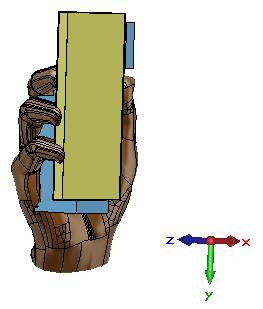
\includegraphics[width=\linewidth, height=4cm, keepaspectratio]{img/tech_sol/usereff_intro/usereff_onehand}
        \caption{Data mode.}
        \label{fig:usereff_onehand}
    \end{subfigure}
    \hfill
    \begin{subfigure}[b]{0.24\linewidth}
        \centering
        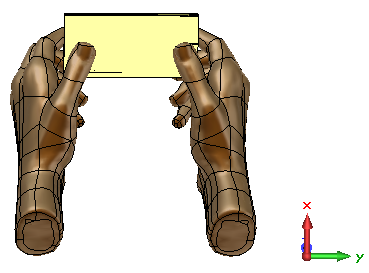
\includegraphics[width=\linewidth, height=4cm, keepaspectratio]{img/tech_sol/usereff_intro/usereff_twohand}
        \caption{Play mode.}
        \label{fig:usereff_twohand}
    \end{subfigure}
    \hfill
    \begin{subfigure}[b]{0.24\linewidth}
        \centering
        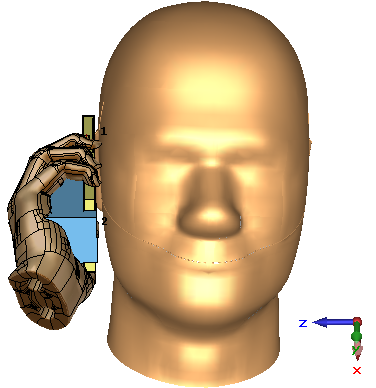
\includegraphics[width=\linewidth, height=4cm, keepaspectratio]{img/tech_sol/usereff_intro/usereff_headhand}
        \caption{Talk mode.}
        \label{fig:usereff_headhand}
    \end{subfigure}
    \hfill
    \begin{subfigure}[b]{0.24\linewidth}
        \centering
        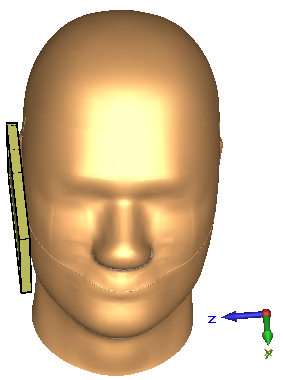
\includegraphics[width=\linewidth, height=4cm, keepaspectratio]{img/tech_sol/usereff_intro/usereff_sar}
        \caption{SAR simulation.}
        \label{fig:usereff_sar}
    \end{subfigure}
    \caption{User effect simulation modes.}
    \label{fig:usereff_intro}
\end{figure}
